\chapter{Implementation of the Trading Systems}
This section provides a comprehensive overview of the two trading system implementations. The first one focuses on the backtesting system, which involves simulating and evaluating strategies in a controlled environment. In this system, historical market data is utilized to test and analyze the performance of various strategies. The second implementation is the live system, designed to execute trades on the Ethereum blockchain using smart contracts. This system operates in real-time and interacts with the live market, allowing for actual trades to be executed based on predefined strategies. Together, these two implementations provide a comprehensive framework for testing, evaluating, and deploying trading strategies, both in simulated environments and on the live blockchain.

\section{Backtesting System}

To develop a resilient backtesting system, a dedicated class was constructed to streamline the process of testing trading strategies. Upon evaluating a particular strategy the \texttt{backtest} function requires \texttt{cointegrated\_pair}, a tuple of the names of the liquidity pools that the strategy is to be evaluated on, \texttt{strategy}, the strategy, and finally, the \texttt{initial\_investment} in ETH. The first argument is required and used to retrieve the relevant historical prices. The second parameter is self-explanatory, the strategy to test. Finally, the inclusion of the initial investment amount as an input parameter enables users to simulate the performance of their strategies with a specific starting capital, it also helps analyze how the various transaction costs affect the ability to trade if any trades do result in a loss. However, the first step is to collect the historical data.

\subsection{Data Collection and Storage}
In order to simulate the market as accurately as possible the system should have access to reliable and accurate historical market data, including price, volume, and other relevant indicators. Therefore, I retrieve all of my data from the Uniswap and Aave protocols' subgraph using the Graph~\cite{noauthor_graph_nodate}. The Graph is a decentralized protocol for indexing and querying blockchain data hence making the data provided 100\% reliable as it indexes directly on the Ethereum blockchain. Subgraphs serve as GraphQL APIs designed to facilitate querying and extracting data from the blockchain. These APIs adhere to a specific schema outlined by the protocol, enabling seamless communication between the protocol and the underlying blockchain. Therefore, I employ the Uniswap V3, Aave V2, and Aave V3 subgraphs to obtain the data required for the backtesting system.
\\[5mm]
The database has the following tables:
\begin{figure}[!htb]
    \centering
    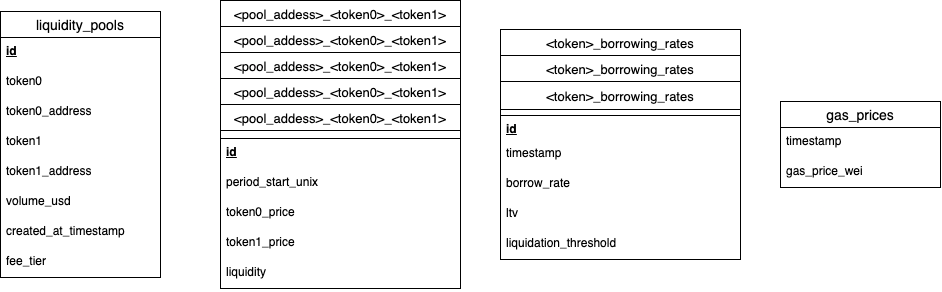
\includegraphics[width=0.8\textwidth]{project/Images/database_tables.png}
    \caption{Tables contained in the database \label{fig:database}}
\end{figure}
The \texttt{liquidity\_pools} contains data about the liquidity pools that exist on Uniswap V3. After obtaining all of the data it is found that it possesses 12,182 liquidity pools. However, a substantial portion of these pools exhibit minimal or negligible trading volume. As a result, a criterion is established to selectively include only those liquidity pools that involve tokens supported by Aave and possess a trading volume exceeding \$10,000,000 (or \$10 million). This filtering condition ensures that the collected and stored data holds significance and relevance for research purposes, as these pools would allow for short selling.
\\[5mm]
Once these pools have been identified, pricing data about each pool that meets this condition is collected again using the Uniswap V3 subgraph. The following shows the GraphQL query:
\vspace{5mm}
\begin{lstlisting}
query ($id: ID!, $prev_max_time: Int!) {
    pool(id: $id) {
        poolHourData(where: {periodStartUnix_gt: $prev_max_time}, orderBy: periodStartUnix, first: 1000) {
            id
            token0Price
            token1Price
            periodStartUnix
            liquidity
            feesUSD
        }
    }
}
\end{lstlisting}
\vspace{5mm}
This query returns an array of dictionaries containing the pre-specified pricing datapoints at a frequency of every hour. Due to the limitations imposed by the subgraph, the results are constrained to a maximum size of 1000 entries. To overcome this limitation and obtain the complete dataset, the query is executed iteratively. The previous maximum time, referred to as \texttt{prev\_max\_time}, is passed as an argument in subsequent queries to fetch the remaining data, i.e. \texttt{prev\_max\_time = hourlyData[-1]['periodStartUnix'] if len(hourlyData) > 0 else prev\_max\_time}. This data is stored in tables of the form \textit{<pool\_address>}\_\textit{<token0>}\_\textit{<token1>}.
\\[5mm]
In a similar manner, obtaining the interest rates for borrowing necessitates the utilization of two of Aave's subgraphs. This requirement arises due to Aave's migration to Version 3 in March 2022, resulting in a transitional period where both Uniswap V3 and Aave V2 were concurrently utilized. The schemas for the two are different, however for the data we require, the borrowing rate, loan-to-value and liquidity threshold, the schema is consistent and the same query can be used:
\vspace{5mm}
\begin{lstlisting}
query ($symbol: String!, $prev_max_time: Int!) {
    reserves(where: {symbol: $symbol}) {
        id
        symbol
        lifetimeBorrows
        baseLTVasCollateral
        reserveLiquidationThreshold
        borrowHistory(
            where: {timestamp_gt: $prev_max_time}, first: 1000, orderBy: timestamp, orderDirection: asc) {
            id
            timestamp
            borrowRate
        }
    }
}
\end{lstlisting}
\vspace{5mm}
During the table initialization process, requests are made to both the V2 and V3 GraphQL endpoints. However, when updating the table, only the V3 endpoint is utilized for sending requests. The data is stored in tables of the form \textit{<symbol>}\_borrowing\_rates, where \textit{<symbol>} are all of the tokens that are present in the liquidity pools that are of interest.
\\[5mm]
To collect the gas price history, the transaction history is queried at each hour since Uniswap migrated to V3. This is because querying in the same as the pricing data and borrowing rate history is too exhaustive as transactions occur every second. Therefore, it is more efficient to query at each hour with a window to retrieve the gas price at the closest hour as follows:
\vspace{5mm}
\begin{lstlisting}
query ($min_time: Int!, $max_time: Int!) {
    transactions(where: {timestamp_gt: $min_time, timestamp_lt: $max_time}, first:1000, orderBy: timestamp, orderDirection: asc) {
        id
        timestamp
        gasPrice
    }
}
\end{lstlisting}
\vspace{5mm}
The following pseudocode shows how to fetch the gas price at each hour:

\begin{algorithm}
    \caption{Retrieval of hourly gas prices where $min\_time$ \& $max\_time$ are arguments}\label{alg_gas_price_col}
    \begin{algorithmic}
        \State $rows\_set \leftarrow \{\}$
        \For{$timestamp$ from $min\_time$ to $max\_time + (60 \times 60), step\_size = (60 \times 60)$}
            \State $found\_result \leftarrow False$
            \State $window\_size\_in\_minutes \leftarrow 5$
            \While{$not\ found\_result$}
                \State $transaction\_data \leftarrow$ GraphQL Query with arguments: $\{``min\_time": timestamp - (60 * window\_size\_in\_minutes), ``max\_time": timestamp + (60 * window\_size\_in\_minutes)\}$
                \If{$transaction\_data != 0$}
                    \State $transaction\_data\_sorted = sorted(transaction\_data, key=lambda\ x:abs(timestamp - int(x['timestamp'])))$
                    \State $rows\_set.update({timestamp: (timestamp, transaction\_data\_sorted[0]['gasPrice'])})$
                    \State $found\_result \leftarrow True$
                \Else
                    \State $window\_size\_in\_minutes \leftarrow window\_size\_in\_minutes + 5$
                \EndIf
            \EndWhile
            \State insert $rows\_set[timestamp]$ into \texttt{gas\_prices} table
        \EndFor
    \end{algorithmic}
\end{algorithm}



\subsection{Types of Orders and Execution}


\section{Live Trading}
